\documentclass[margin=2mm]{standalone}
\usepackage{bm}
\usepackage{calligra}
\newcommand{\setfont}[2]{{\fontfamily{#1}\selectfont #2}}
\usepackage{tikz}
\usetikzlibrary{3d}

\usetikzlibrary{calc}
\usetikzlibrary{patterns}
\usetikzlibrary{decorations.text}
\usetikzlibrary{decorations.pathmorphing}
\usetikzlibrary{decorations.markings}

\newcommand{\picturefontsize}{\LARGE}
\newcommand{\pictureLineWidth}{0.8mm}

\begin{document}
% For every picture that defines or uses external nodes, you'll have to
% apply the 'remember picture' style. To avoid some typing, we'll apply
% the style to all pictures.
\tikzstyle{every picture}+=[remember picture]
\tikzstyle{na} = [baseline=-.5ex]

\begin{tikzpicture}%[show background grid]% every node/.style={draw,outer sep=0pt,thick}]

\tikzstyle{ground}=[fill, pattern=north west lines, draw=none]

\newcommand{\CoG}[1]{%
    \draw (#1) circle[radius=14pt, black, line width = 1pt];%
    \filldraw[black, line width=0.1pt] (#1) ++( 14pt,   0) -- ++(-28pt,     0);%
    \filldraw[black, line width=0.1pt] (#1) ++(   0, 14pt) -- ++(    0, -28pt);%
    \filldraw[black, line width=0.1pt] (#1) -- ++( 14pt,0) arc (  0:90 :14pt) -- cycle;%
    \filldraw[black, line width=0.1pt] (#1) -- ++(-14pt,0) arc (180:270:14pt) -- cycle;%
    %\node[anno-ptr, xshift=5pt, yshift=-5pt, anchor = north west] at
    %(#1) {CoM};%
}
\newcommand{\CoGsmall}[1]{%
    \draw (#1) circle[radius=4pt, black, line width = 1pt];%
    \filldraw[black, line width=0.1pt] (#1) ++( 5pt,   0) -- ++(-10pt,     0);%
    \filldraw[black, line width=0.1pt] (#1) ++(   0, 5pt) -- ++(    0, -10pt);%
    \filldraw[black, line width=0.1pt] (#1) -- ++( 3pt,0) arc (  0:90 :3pt) -- cycle;%
    \filldraw[black, line width=0.1pt] (#1) -- ++(-3pt,0) arc (180:270:3pt) -- cycle;%
    %\node[anno-ptr, xshift=5pt, yshift=-5pt, anchor = north west] at
    %(#1) {CoM};%
}

% Put the graphic inside a node. This makes it easy to place the
% graphic and to draw on top of it.
% The above right option is used to place the lower left corner
% of the image at the (0,0) coordinate.
\node [inner sep=0pt,above right] {
    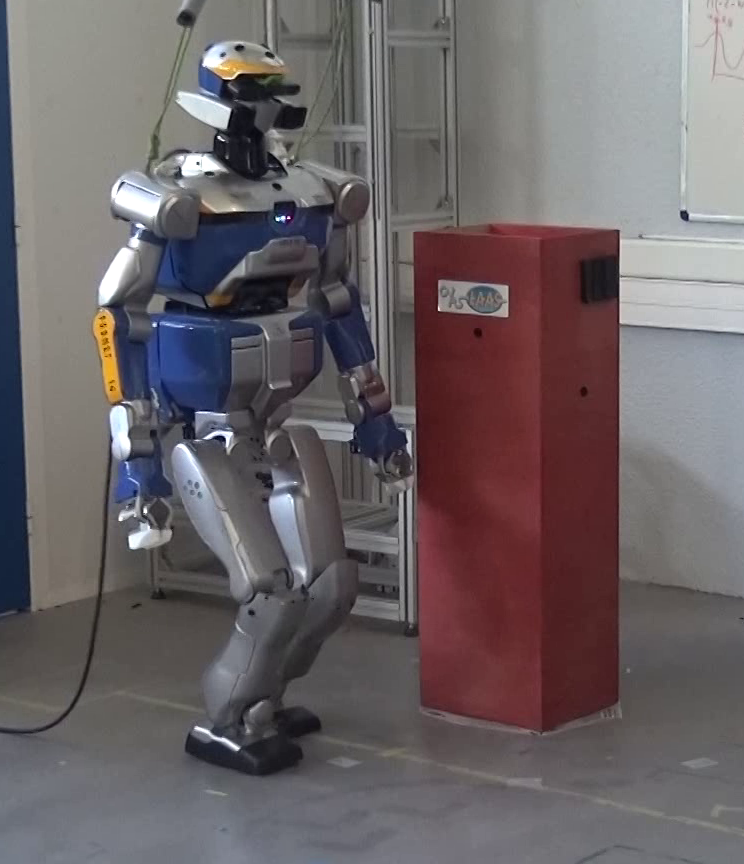
\includegraphics[width=1.0\linewidth]{../HRP2-obstacle-avoidance-2.png}
};
% coordinate system
\def\cosxaxis{1.0}
\def\sinxaxis{0.0}
\def\cosyaxis{ 0.866025403784}
\def\sinyaxis{ 0.5}
\def\coszaxis{0.0}
\def\sinzaxis{1.0}

% define origin
\coordinate (origin) at (0.0, 0.0);

% define origin of world
\coordinate (cos_ori) at (1.0, 1.0);
%\fill[magenta] (cos_ori) circle (2pt); % show origin

\def\ax_length{2.5}
\path (cos_ori) ++ ( \ax_length * \cosxaxis, \ax_length * \sinxaxis) coordinate (cos_x);
\def\ax_length{1.75}
\path (cos_ori) ++ ( \ax_length * \cosyaxis, \ax_length * \sinyaxis) coordinate (cos_y);
\def\ax_length{2.0}
\path (cos_ori) ++ ( \ax_length * \coszaxis, \ax_length * \sinzaxis) coordinate (cos_z);

\draw [->, line width=\pictureLineWidth, orange!50] (cos_ori) -- (cos_x);
\draw [->, line width=\pictureLineWidth, orange!50] (cos_ori) -- (cos_y);
\draw [->, line width=\pictureLineWidth, orange!50] (cos_ori) -- (cos_z);

\node[draw=none,text=orange!50, above left]  at (cos_ori) {\picturefontsize $\mathcal W$};
\node[draw=none,text=orange!50, below      ] at (cos_x) {\picturefontsize $x$};
\node[draw=none,text=orange!50,       right] at (cos_y) {\picturefontsize $y$};
\node[draw=none,text=orange!50, below left] at (cos_z) {\picturefontsize $z$};

% draw handrail
%\coordinate (p3_pos) at (5.8, 4.6);
%\node[ ground, pattern color=black, anchor=north,
%       minimum width=1.0cm, minimum height=0.5cm,
%       rotate around={30:(p3_pos.center)}
%] (limit) at (p3_pos) {};
%\node[ fill=white, draw=none, anchor=south,
%       minimum width=1.0cm, minimum height=0.5cm,
%       rotate around={30:(p3_pos.center)}
%] at (limit.north) {};
%\node[ fill=white, draw=none, anchor=north,
%       minimum width=1.0cm, minimum height=0.5cm,
%       rotate around={30:(limit.south)}
%] at (limit.south) {};
%\draw [thick, black] (limit.north west) -- (limit.north east);

% COM
% define position of CoM
\coordinate (com_pos) at (4.5, 8.0);
%\fill[magenta] (com_pos) circle (2pt); % show origin
%\path (com_pos) ++ ( 0.0, 0.0) ++ (-0.4, -0.4) node [draw=none] (com_txt) {$CoM$};

% Inertia Ellipsoid
% define size of inertia ellipsoid (ie) around CoM
%\draw[name=ellipse, line width=\pictureLineWidth, rotate around={80:(com_pos.center)}, black!30        ] (com_pos) circle[x radius = 6.0, y radius = 1.75];
%\draw[name=ellipse, thin, rotate around={85:(com_pos.center)}, black!10, dashed] (com_pos) circle[x radius = 0.5, y radius = 1.75];
%\draw[name=ellipse, thin, rotate around={85:(com_pos.center)}, black!10, dashed] (com_pos) circle[x radius = 3.0, y radius = 0.25];

% draw axes
%\draw[thin, rotate around={85:(com_pos.center)}, black!20] (com_pos)  ++ (-3.00, 0.00) --++ (2*3.00,   0.00);
%\draw[thin, rotate around={85:(com_pos.center)}, black!20] (com_pos)  ++ ( 0.00,-1.75) --++ (  0.00, 2*1.75);
%\draw[thin, rotate around={85:(com_pos.center)}, black!20] (com_pos)  ++ (-0.50, 0.25) --++ (2*0.50,-2*0.25);

% doit 3D style\pictureLineWidth
%\draw[line width=\pictureLineWidth, rotate around={80:(com_pos.center)}, black!10, dashed] ($(com_pos) + ( 0:6.0 and 1.7)$) arc (  0: 180:6.0 and 0.7);% left half of the left ellipse

%\draw[line width=\pictureLineWidth, rotate around={80:(com_pos.center)}, black!10, dashed] ($(com_pos) + (90:0.5 and 1.75)$) arc ( 90:-90:0.5 and 1.75);% left half of the left ellipse
%\draw[line width=\pictureLineWidth, rotate around={80:(com_pos.center)}, black!10        ] ($(com_pos) + (90:0.5 and 1.75)$) arc ( 90:270:0.5 and 1.75);% left half of the left ellipse

% add COM coordinate system

\def\cosxaxis{1}
\def\sinxaxis{0}
\def\cosyaxis{0.87557768}
\def\sinyaxis{0.48307734}
\def\coszaxis{0}
\def\sinzaxis{1}

\def\ax_length{1.5}
\path (com_pos) ++ ( \ax_length * \cosxaxis, \ax_length * \sinxaxis) coordinate (com_x);
\def\ax_length{1.375}
\path (com_pos) ++ ( \ax_length * \cosyaxis, \ax_length * \sinyaxis) coordinate (com_y);
\def\ax_length{1.75}
\path (com_pos) ++ ( \ax_length * \coszaxis, \ax_length * \sinzaxis) coordinate (com_z);

\draw [->, line width=\pictureLineWidth, magenta!70] (com_pos) -- (com_x);
\draw [->, line width=\pictureLineWidth, magenta!70] (com_pos) -- (com_y);
\draw [->, line width=\pictureLineWidth, magenta!70] (com_pos) -- (com_z);

\node[thick,draw=none, text=magenta!70, below left] at (4.5, 9.1) {\picturefontsize $\mathcal C$};
\node[thick,draw=none, text=magenta!70, below     ] at (com_x) {\picturefontsize $x$};
\node[thick,draw=none, text=magenta!70,             right] at (com_y) {\picturefontsize $y$};
\node[thick,draw=none, text=magenta!70,       right] at (com_z) {\picturefontsize $z$};

% draw CoM
\CoG{com_pos}
\coordinate (obstacle_psa) at (4.75, 2.1);
\coordinate (obstacle_psa2) at (6.75, 2.5);
%

%\begin{scope}[canvas is xy plane at z=0]
%     \draw[green] (0,0) circle (1cm);
%     \draw (-1,0) -- (1,0) (0,-1) -- (0,1);
%\end{scope}

\draw[line width=\pictureLineWidth, green!50] ($(obstacle_psa)$) arc (-170:-38:4 and 1.1);% left half of the left ellipse
%\draw[line width=\pictureLineWidth, black!10] ($(obstacle_psa2)$) arc ( 120:160:5 and 0.15);% left half of the left ellipse
\draw[line width=\pictureLineWidth, red!50] ($(obstacle_psa2)$) arc ( -160:-30:2.0 and 0.7);% left half of the left ellipse
\draw[<->,thick,color=white] (8.1,2.0) -- (8.1,1.3)
  node[right ,text width=3cm,text ragged,midway]
  {
    \textcolor{white}{\picturefontsize Safety Area}
  };
\draw[->,line width=\pictureLineWidth,color=blue!40] ($(obstacle_psa) $) -- ($(obstacle_psa)+(1.4,-0.4)$ ) 
  node[above right ,text width=3cm,text ragged,midway]
  {
    \textcolor{blue!40}{\picturefontsize $\bm{\setfont{calligra}{v}}^{ref}_k$}
  };
%\draw[step=1.0,very thin,black!20] (0,0) grid (12,14);
\end{tikzpicture}
\end{document}










